\chapter{Trägheitsmoment}
\label{v:2}

\etutorhint{Bitte führen Sie zuerst den Pohl-Versuch durch. Damit versuchen wir sicherzustellen, dass nicht gleichzeitig Pohl und e/m im selben Raum laufen. Für den Versuch e/m muss der Raum komplett abgedunkelt sein...}

In diesem Versuch lernen Sie die Grundlagen der Rotation starrer (nicht verformbarer) Körper kennen.\\
Zur Vorbereitung ist es nützlich, sich den theoretischen Hintergrund von Versuch \ref{v:1} anzuschauen, wenn Sie diesen Versuch noch nicht gemacht haben.
% Zusätzlich: Schwingen mit angezogenen Armen beim Laufen, um Rotationsenergie zu reduzieren,
% Pirouette beim Eiskunstlauf
% --> Haben wir einen Probekörper an einer langen Achse?
% --> Drehmoment in die Anleitung?
%------------------------------------------------
\section{Stichworte}
%------------------------------------------------
Lineare (harmonische) Schwingungen; Drehschwingungen; Winkelgeschwindigkeit; Drehimpulserhaltung; Trägheitsmoment; Drehmoment; Steinerscher Satz; 
%
%------------------------------------------------
\section{Literatur}
%------------------------------------------------
Gehrtsen, Kapitel 1.4.2/3, 2.1 und 2.2; Demtröder, Kapitel 2.4.1, 2.8, 4.5, 5.5
%
%------------------------------------------------
\section{Anwendungsbeispiele}
%------------------------------------------------
%
Die Rotation starrer Körper und die dabei verwendeten Trägheitsmomente der Körper beschreiben nicht nur die Vorgänge bei der Rotation eines Spielzeugkreisels oder des Gyroskopstabilisators von Schiffen, sondern auch die Rotation von Atomen und Molekülen, bei denen manche Achsen (Hauptträgheitsachsen) bevorzugt sind. Die Rotation der Erde um ihre eigene Achse wird ebenso beschrieben wie die Umdrehung von Fahrradreifen oder die Rotation des Arms im Schultergelenk.
%
%------------------------------------------------
\section{Theoretischer Hintergrund}
%------------------------------------------------

\subsection{Das Trägheitsmoment}

Wir betrachten einen starren Körper, der um eine feststehende Achse rotiert. Um die gesamte kinetische Energie des Körpers aufgrund seiner Rotation berechnen zu können, unterteilen wir den Körper in sehr kleine würfelförmige Elemente, die die kleine Masse $dm_i$ (\textit{Massenelement}) haben. Diese Massenelemente haben den senkrechten Abstand $r_i$ von der Drehachse. Somit können wir die gesamte kinetische Energie schreiben als:
\begin{equation}
\label{Gl:Erot_sum}
E_{rot} = \frac{1}{2} \sum{dm_i v_i^2} = \frac{1}{2} \omega^2 \sum{dm_i r_i^2}
\end{equation}
mit der Winkelgeschwindigkeit $\omega = r\cdot v$.\\
Bei einem kontinuierlichen Körper können wir das Massenelement $dm_i$ über die Dichte des Körpers ausdrücken als $dm_i = \rho\cdot dV$. Lassen wir nun die Würfel, aus denen wir den Körper zusammensetzen, unendlich klein (infinitesimal) werden, so geht die Summe in Gleichung \ref{Gl:Erot_sum} in das Integral über:
\begin{equation}
\label{Gl:Erot_integral}
E_{rot} = \frac{1}{2}\omega^2\int{\rho r^2 dV}
\end{equation}
%
Wir lassen die Dichte $\rho$ unter dem Integral, weil sie von Ort zu Ort verschieden sein kann. \\

Betrachten wir den in Gleichung \ref{Gl:Erot_integral} auftretenden Ausdruck
\begin{equation}
\label{Gl:Traegheitsmoment}
J = \sum{dm_i r_i^2} = \int{\rho r_i^2 dV} \; ,
\end{equation}
das \textit{Trägheitsmoment} des Körpers. Er besagt, dass sich die einzelnen Masseteile in der Rotation umso mehr auswirken, je weiter sie von der Rotationsachse entfernt sind. Dementsprechend hängt $J$ sowohl von der genauen Form des Körpers ab, als auch davon, wo die Rotationsachse des Körpers liegt. Beispielsweise betragen die Trägheitsmoment einiger einfacher Körper:
\begin{itemize}
\item Kreisscheibe oder Zylinder, Achse durch die Symmetrieachse:
	\begin{equation} \label{eq:J_Zylinder}
	J = \frac{1}{2} MR^2
	\end{equation}
\item Hohlzylinder (Innenradius $R_i$, Aussenradius $R_a$), Achse durch Symmetrieachse:
	\begin{equation}
	J = \frac{1}{2} M(R_a^2 + R_i^2)
	\end{equation}
\item Vollkugel, Achse durchs Zentrum:
	\begin{equation}
	J = \frac{2}{5} MR^2
	\end{equation}
\item Würfel der Kantenlänge $a$, für jede Achse, die durch den Schwerpunkt geht:
	\begin{equation}
	J = \frac{1}{6} Ma^2
	\end{equation}
\item Stab der Länge $L$, Achse senkrecht zum Stab durch den Schwerpunkt:
	\begin{equation}
	J = \frac{1}{12} ML^2
	\end{equation}
\end{itemize}

\subsection{Der Steiner'sche Satz}

Wenn man das Trägheitsmoment eines Körpers in Bezug auf eine durch seinen Schwerpunkt gehende Achse $A'$ kennt, liefert der \textit{Steiner'sche Satz} das Trägheitsmoment in Bezug auf eine andere dazu parallele Achse $A$. Der Abstand zwischen den beiden Achsen sei $a$:
\begin{equation}
\label{Gl:Steiner}
J_A = J_{A'} + Ma^2
\end{equation}
%
Wie man leicht nachrechnen kann, ergibt sich damit für das Trägheitsmomentes eines Stabes, bei dem die Drehachse einen Abstand $b$ zum Schwerpunkt hat:
\begin{equation} \label{eq:J_Stab-Steiner}
J = \frac{1}{12}ML^2 + mb^2 \, .
\end{equation}

\subsection{Drehschwingungen}

Eine Spiralfeder übt ein Drehmoment $\vec{T}$ aus, das dem Auslenkungswinkel aus der Ruhelage proportional und entgegengerichtet ist:
\begin{equation}
 \vec{T} = -D^*\cdot\varphi\cdot \hat{e}_{\varphi} \; .
\end{equation}
$D^*$ heißt \textit{Winkelrichtgröße} oder \textit{Richtmoment} und ist eine Eigenschaft der gewählten Feder. Unter der Wirkung eines solchen Moments führt ein an der Spiralfeder befestigter Körper entsprechend der Bewegungsgleichung
\begin{equation}
 \vec{T} = -D^*\cdot\varphi\cdot \hat{e}_{\varphi} = \dot{\vec{L}} = J\ddot{\varphi}\cdot\hat{e}_{\varphi}
\end{equation}
Drehschwingungen aus. Das Symbol $\dot{\vec{L}}$ bezeichnet dabei die zeitliche Änderung des Dreh- impulses $\vec{L} = m\cdot \vec{r}\times\vec{p}$. Analog zu den Translationsschwingungen aus Versuch 1 ergibt sich für die Frequenz der Schwingung:
\begin{equation}
 \omega = \frac{2\pi}{T} = \sqrt{\frac{D^*}{J}}
\end{equation}
$T$ ist hierbei die Schwingungsdauer.

%------------------------------------------------
\section{Fragen zur Vorbereitung}
%------------------------------------------------

\begin{enumerate} 
 %
% \item Was soll heute im Praktikum gemessen werden? Warum?
 %
 \item Welche Größen beschreiben eine Drehbewegung?
 %
 \item Wie lautet der Steiner'sche Satz?
 %
 \item Was ist eine harmonische Schwingung?
 %
 \item Gilt die Energie-Erhaltung bei der Spiralfeder? Beschreiben Sie die Energieverhältnisse während der Drehschwingung.
 %
 \item Wie ist das Drehmoment definiert? (Formel und Einheit)
 % 
 \item Wie ist der Drehimpuls definiert? (Formel und Einheit)
 %
\end{enumerate} 

%------------------------------------------------
\section{Durchführung} 
%------------------------------------------------

\begin{enumerate}
 %
	\begin{minipage}{0.6\textwidth}
		\item Der Halter wird so eingespannt, dass die Drehachse horizontal liegt. An der aufgesteckten Scheibe wird die Schnur befestigt. Für verschiedene an die Schnur gehängte Massen (m = 10, 15, 20, 30, 40~g) wird der Winkelausschlag $\Phi$ im Uhrzeigersinn und entgegengesetzt abgelesen. Achten Sie darauf, dass die Feder nicht an den Rahmen anschlägt!
		%
		\item Messen Sie den Radius $r$ der Scheibe.
		%
		\item Tragen Sie für jede Masse $M$ den entsprechenden Winkelausschlag $\Phi$ im Bogenmaß auf. Bilden Sie dazu jeweils den Mittelwert aus der Auslenkung im und gegen den Uhrzeigersinn und bestimmen Sie die Fehler auf diese Mittelwerte.
		%
		\item Nehmen Sie die Scheibe ab. Lösen Sie die Montageschraube und ziehen Sie die Halterung der Drehachse aus dem Stativ, um sie anschließend so zu montieren, dass die Drehachse vertikal liegt.
		%
		\item Messen Sie bei vertikaler Lage der Drehachse für jeden Versuchskörper (Vollzylinder, Hohlzylinder, Kugel, Quader, Stab) dreimal die Zeit für jeweils 10 Drehschwingungen. Beim Würfel sind zwei verschiedene Drehachsen zu wählen. Beim Stab werden zwei parallele Achsen gewählt; eine davon geht durch den Schwerpunkt, die andere liegt am Ende des Stabes.
		%
	\end{minipage}\hfill
	%
	\begin{minipage}{0.35\textwidth}
		\centering
		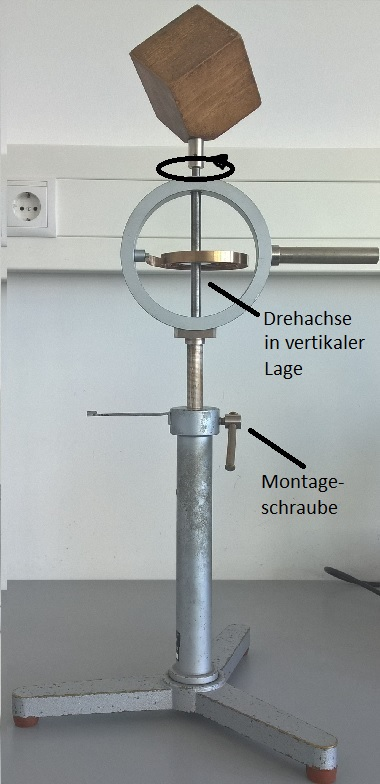
\includegraphics[width=0.9\textwidth]{Abbildungen/Traegheitsmoment.jpg}
	\end{minipage}

		 \item Messen Sie die geometrischen Daten der Versuchskörper (Radien, Kantenlängen). Die Masse $M$ der Versuchskörper muss auch gemessen werden, da die jeweils auf den Körpern  angegebenen Massen nicht stimmen.
\end{enumerate}

%------------------------------------------------
\section{Auswertung} 
%------------------------------------------------
\etodo{Musterauswertung}

\begin{hint}
	Bitte fertigen Sie die Graphen in der folgenden Auswertung per Hand auf Millimeterpapier an.
\end{hint}

\begin{enumerate}
 %
 \item Berechnen Sie aus der Steigung der Funktion $\Phi (M)$ das Richtmoment (Winkelrichtgröße) $D^*$ der Feder nach der Formel:
 \begin{equation}
 D^* = \frac{M}{\Phi}\cdot g\cdot r \; .
 \end{equation}
 Berechnen Sie auch den Fehler auf das Richtmoment.
 %
 \item Berechnen Sie die Trägheitsmomente $J_{exp}$ der verschiedenen Versuchskörper aus den gemessenen Schwingungsdauern $T$. Benutzen Sie:
 \begin{equation}
 T = 2\pi\sqrt{\frac{J_{exp}}{D^*}} \; .
 \end{equation}
 Fehlerrechnung nicht vergessen!
 %
 \item Berechnen Sie aus den geometrischen Daten der Versuchskörper die theoretischen Trägheitsmomente $J_{th}$ inklusive ihrer Fehler. Benutzen Sie die Gleichungen \ref{eq:J_Zylinder} bis \ref{eq:J_Stab-Steiner}.
 %
 \item Vergleichen Sie die gemessenen und berechneten Werte $J_{exp}$ und $J_{th}$ für die verschiedenen Versuchskörper. Geben Sie eine Erklärung für mögliche Differenzen zwischen den Werten.
 %
\end{enumerate}